\documentclass[12pt, twoside]{article}
\usepackage[letterpaper, margin=1in, headsep=0.5in]{geometry}
\usepackage[english]{babel}
\usepackage[utf8]{inputenc}
\usepackage{amsmath}
\usepackage{amsfonts}
\usepackage{amssymb}
\usepackage{tikz}
\usetikzlibrary{quotes, angles}
\usepackage{graphicx}
\usepackage{enumitem}
\usepackage{multicol}

\newif\ifmeta
\metatrue %print standards and topics tags

\title{Regents Geometry}
\author{Chris Huson}
\date{September 2020}

\usepackage{fancyhdr}
\pagestyle{fancy}
\fancyhf{}
\renewcommand{\headrulewidth}{0pt} % disable the underline of the header
\raggedbottom


\fancyhead[LE]{\thepage}
\fancyhead[RO]{\thepage \\ Name: \hspace{4cm} \,\\}
\fancyhead[LO]{BECA / Dr. Huson / Geometry Unit 2 Angles\\13 October 2020}

\begin{document}

\subsubsection*{2.1 Worksheet Angle terminology}
\begin{enumerate}
\item I have a compass, ruler, protractor, notebook, and folder (circle one). Yes \qquad No
    \vspace{0.25cm}

\item Write the appropriate name for the type of angle depending on its measure in degrees. (acute, right, obtuse, or straight)
    \begin{enumerate}
      \item $m\angle = 90$ : \rule{4cm}{0.15mm} \bigskip
      \item $90 < m\angle < 180$ : \rule{4cm}{0.15mm} \bigskip
      \item $0< m\angle < 90$ : \rule{4cm}{0.15mm} \bigskip
      \item $m\angle = 180$ : \rule{4cm}{0.15mm} \bigskip
    \end{enumerate}

\item Write down the name of the given angle three different ways.\\
    \begin{tikzpicture}
      \draw
        (3,-1) coordinate (a) node[right] {A}
        -- (0,0) coordinate (b) node[left] {B}
        -- (2,2) coordinate (c) node[above right] {C}
        pic["1", <->, draw=black, angle eccentricity=1.2, angle radius=1cm]
        {angle=a--b--c};
    \end{tikzpicture}

\item Points that are all located on the same plane are $\rule{4cm}{0.15mm}$.

\item Write down the name of the angle shown in the diagram below using proper geometric notation.
    \begin{center}
    \begin{tikzpicture}[scale=2]
      \draw [->, thick] (0,0)--(4,3);
      \draw [->, thick] (0,0)--(5,-1);
      \draw [fill] (2.66666,2) circle [radius=0.05] node[above left ]{$D$};
      \draw [fill] (0,0) circle [radius=0.05] node[above left]{$E$};
      \draw [fill] (4,-0.8) circle [radius=0.05] node[above]{$F$};
    \end{tikzpicture}
    \end{center}
    Find the measure of the angle in degrees with a protractor.

\newpage
\item Given $\overline{ABC}$, $AB=3x-2$, $BC=x+11$, $AC=29$. Find ${AB}$. Show each step:\\ \vspace{0.5cm}
    \begin{flushright}
      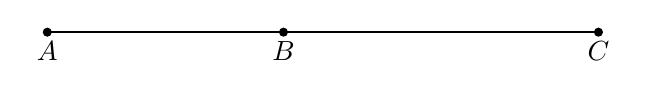
\begin{tikzpicture}
         \draw [-, thick] (0,0)--(7,0);
         \draw [fill] (0,0) circle [radius=0.05] node[below]{$A$};
         \draw [fill] (3,0) circle [radius=0.05] node[below]{$B$};
         \draw [fill] (7,0) circle [radius=0.05] node[below]{$C$};
      \end{tikzpicture}
    \end{flushright}
      %\vspace{1cm}
    \begin{enumerate}
      \item Sketch and label the situation
      \item Write a geometric equation
      %\begin{flushright} Segment addition\\ postulate \end{flushright}
      \item Substitute algebraic values and solve
      %\item Solve for the unknown
      \vspace{3cm}
      \begin{flushright} $x=$ \rule{1cm}{0.15mm} \end{flushright}
      \item Answer the question
      \begin{flushright} $AB=$ \rule{1cm}{0.15mm} \end{flushright}
      \item Check your answer
    \end{enumerate} \vspace{2cm}

\item Spicy: Given isosceles $\triangle ABC$ with $\overline{AC} \cong \overline{BC}$. $AC=5x+7$ and $BC=3x+17$. \\ Find $AC$.\\[0.5cm]
    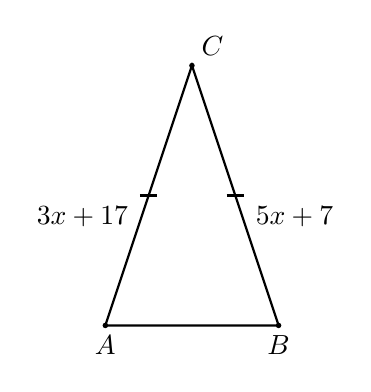
\begin{tikzpicture}[scale=0.55]
      \draw [thick](0,0)--(4,0)--(2,6)--(0,0);
      \draw [fill] (0,0) circle [radius=0.05] node[below]{$A$};
      \draw [fill] (4,0) circle [radius=0.05] node[below]{$B$};
      \draw [fill] (2,6) circle [radius=0.05] node[above right]{$C$};
      \draw [thick] (0.8,3)--(1.2,3); %tick mark
      \draw [thick] (2.8,3)--(3.2,3); %tick mark
      \node [right] at (3.25,2.5){$5x+7$};
      \node [left] at (0.75,2.5){$3x+17$};
    \end{tikzpicture}

\end{enumerate}
\end{document}